\chapter{Node.js}

\section{Ejemplos}

Esta práctica contiene cinco ejemplos que debemos ejecutar antes de proceder a escribir el ejercicio.
Tanto los ejemplos como el ejercicio requieren que las dependencias se instalen localmente al proyecto.
Para ello, podemos usar tanto \texttt{npm} como \texttt{yarn}:

\begin{lstlisting}[language=sh]
npm install  # Instalar las dependencias con npm
yarn install # Instalar las dependencias con yarn
\end{lstlisting}

Es importante tener en cuenta que el programa que elijamos para instalar las dependencias debería ser el programa que utilicemos para ejecutar los ejemplos y el ejercicio.
No es estrictamente necesario, pero usar ambos programas indistintamente generará un aviso indicando que el fichero \texttt{(package|yarn).lock} ha sido generado por un programa ajeno al ejecutante.

La ejecución de los ejemplos se ha simplificado añadiendo órdenes de ejecución al fichero \texttt{package.json}.
Es importante tener en cuenta que estas órdenes utilizan el programa \texttt{ts-node} en lugar de \texttt{node} para compilar y ejecutar los ficheros, que están escritos en TypeScript en lugar de en JavaScript.
He elegido escribir los ejercicios en este lenguaje porque es una extensión de JavaScript que debe compilarse antes de ser ejecutado y ello permite detectar una enorme cantidad de errores durante la escritura del programa.

\subsection{¡Hola, mundo!}

\begin{lstlisting}[language=sh]
yarn hola-mundo
\end{lstlisting}

Este ejemplo presenta un comportamiento muy sencillo.
Primero se ejecuta el programa con la orden especificada y luego ha de abrirse la dirección \texttt{127.0.0.1:8080} en el navegador.
En él se nos mostrará la cadena \texttt{Hola mundo}, que es la que hemos enviado mediante la llamada a \texttt{response.write()}.

\subsection{Calculadora}

\begin{lstlisting}[language=sh]
yarn calculadora
\end{lstlisting}

Con este ejemplo practicamos llamadas al servidor mediante argumentos incrustrados en la url.
Para ello debemos conectarnos a la dirección \texttt{127.0.0.1:8080} y añadir los argumentos de la operación que queremos realizar en el siguiente orden:

\begin{itemize}
	\item
		\texttt{operacion: string}
	\item
		\texttt{val1: number}
	\item
		\texttt{val2: number}
\end{itemize}

Aquí empezamos a apreciar las ventajas de utilizar TypeScript, pues la función que ejecuta las operaciones obliga al resto del programa a pasarle los argumentos con el tipo correcto y a devolver únicamente los tipos requeridos al especificarlos en la cabecera:

\begin{lstlisting}
function Calcular (operacion: string, val1: number, val2: number): number | string
\end{lstlisting}

\pagebreak

Las operaciones permitidas son \texttt{sumar}, \texttt{restar}, \texttt{multiplicar} y \texttt{dividir}, por lo que podemos realizar llamadas a la calculadoras con urls como las siguientes:

\begin{lstlisting}
http://127.0.0.1:8080/sumar/2/3
http://127.0.0.1:8080/restar/4/2
http://127.0.0.1:8080/multiplicar/7/5
http://127.0.0.1:8080/dividir/20/7
\end{lstlisting}

Al igual que en ejercicios anteriores, el resultado de la operación se muestra en el navegador.

\subsection{Calculadora web}

\begin{lstlisting}[language=sh]
yarn calculadora-web
\end{lstlisting}

Este ejemplo funciona de forma similar al anterior pero con la particularidad de que las peticiones al servidor no se generan desde la url sino desde un formulario manipulable por el usuario, de forma que los resultado se muestran debajo de éste.

\begin{figure}[!ht]
\begin{center}
	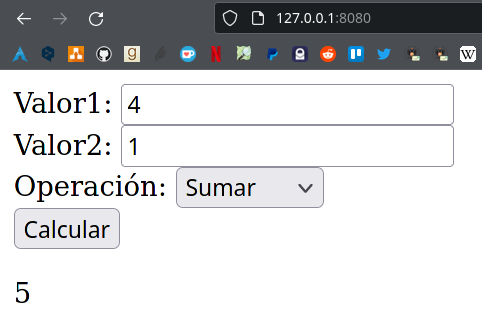
\includegraphics[scale=0.5]{node_calculadora_web}
\end{center}
\caption{Formulario de la calculadora web.}
\end{figure}

El cliente envía al servidor peticiones REST y éste responde con el resultado de la operación.

\subsection{Connections}

\begin{lstlisting}[language=sh]
yarn connections
\end{lstlisting}

En este ejemplo abrimos una conexión \texttt{WebSocket} usando la interfaz implementada por \texttt{socket.io}.
El funcionamiento de este ejemplo es muy sencillo.
Cuando el servidor se enciende espera a que se conecte un cliente y muestra por consola que lo ha hecho.
Lo mismo ocurre cuando se desconecta.
Al conectarse el cliente, el servidor le envía un mensaje que reza \texttt{¡Hola, Cliente!}.
Si cerramos el servidor cuando el cliente sigue encendido, éste lo detecta e imprime \texttt{¡El servicio ha dejado de funcionar!}.

\begin{figure}[!ht]
\begin{center}
	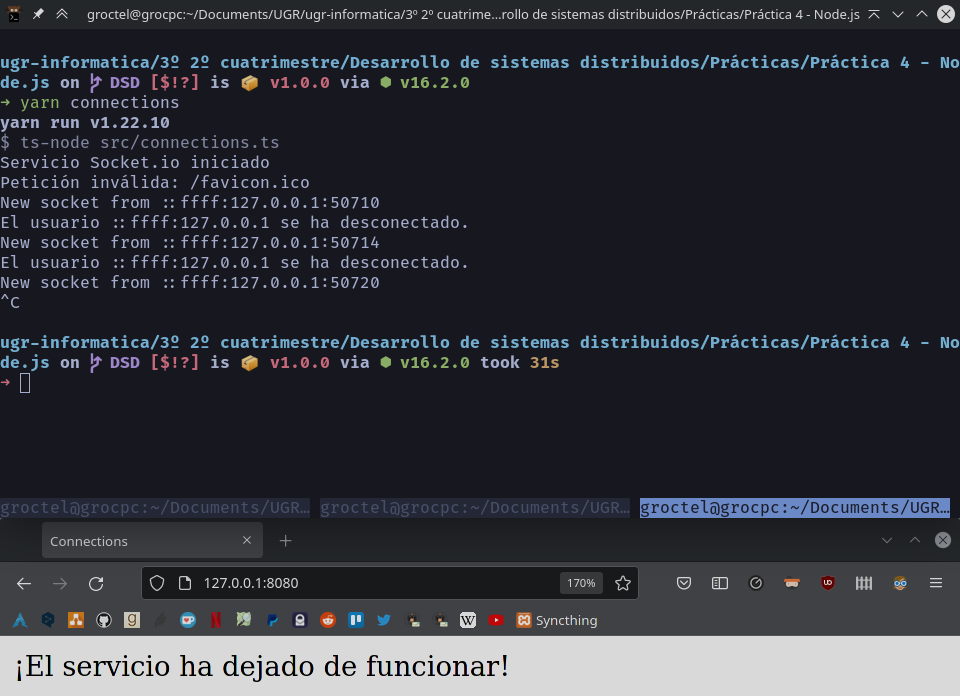
\includegraphics[scale=0.27]{node_connections}
\end{center}
\caption{Interacción del cliente y el servidor.}
\end{figure}

\subsection{Mongo test}

\begin{lstlisting}[language=sh]
yarn mongo-test
\end{lstlisting}

En este ejemplo hacemos una primera aproximación al uso de MongoDB mediante node.js.
Para poder ejecutar este ejemplo es necesario tener instalado \href{https://aur.archlinux.org/packages/mongodb-bin/}{\texttt{mongodb-bin}} e iniciar el servicio correspondiente:

\begin{lstlisting}[language=sh]
systemctl start mongodb
\end{lstlisting}

También es necesario tener una base de datos llamada \texttt{mydb} en el sistema.

La ejecución de este ejemplo también es bastante sencilla.
Primero se comprueba si existe una colección (una tabla) llamada \texttt{mycoll}.
Si existe, se elimina antes de crearla, de forma que la salida mostrada por el navegador sea única de la sesión.
Tras ello, el sistema conecta el cliente y el servidor usando \texttt{socket.io} y va almacenando las direcciones de los clientes conectados en la colección.
Cuando el cliente se conecta, muestra en pantalla una lista con todos los clientes que se han conectado esta sesión con la misma dirección que él.

\section{Ejercicio}

\begin{lstlisting}[language=sh]
yarn domotica
\end{lstlisting}

\begin{figure}[!ht]
\begin{center}
	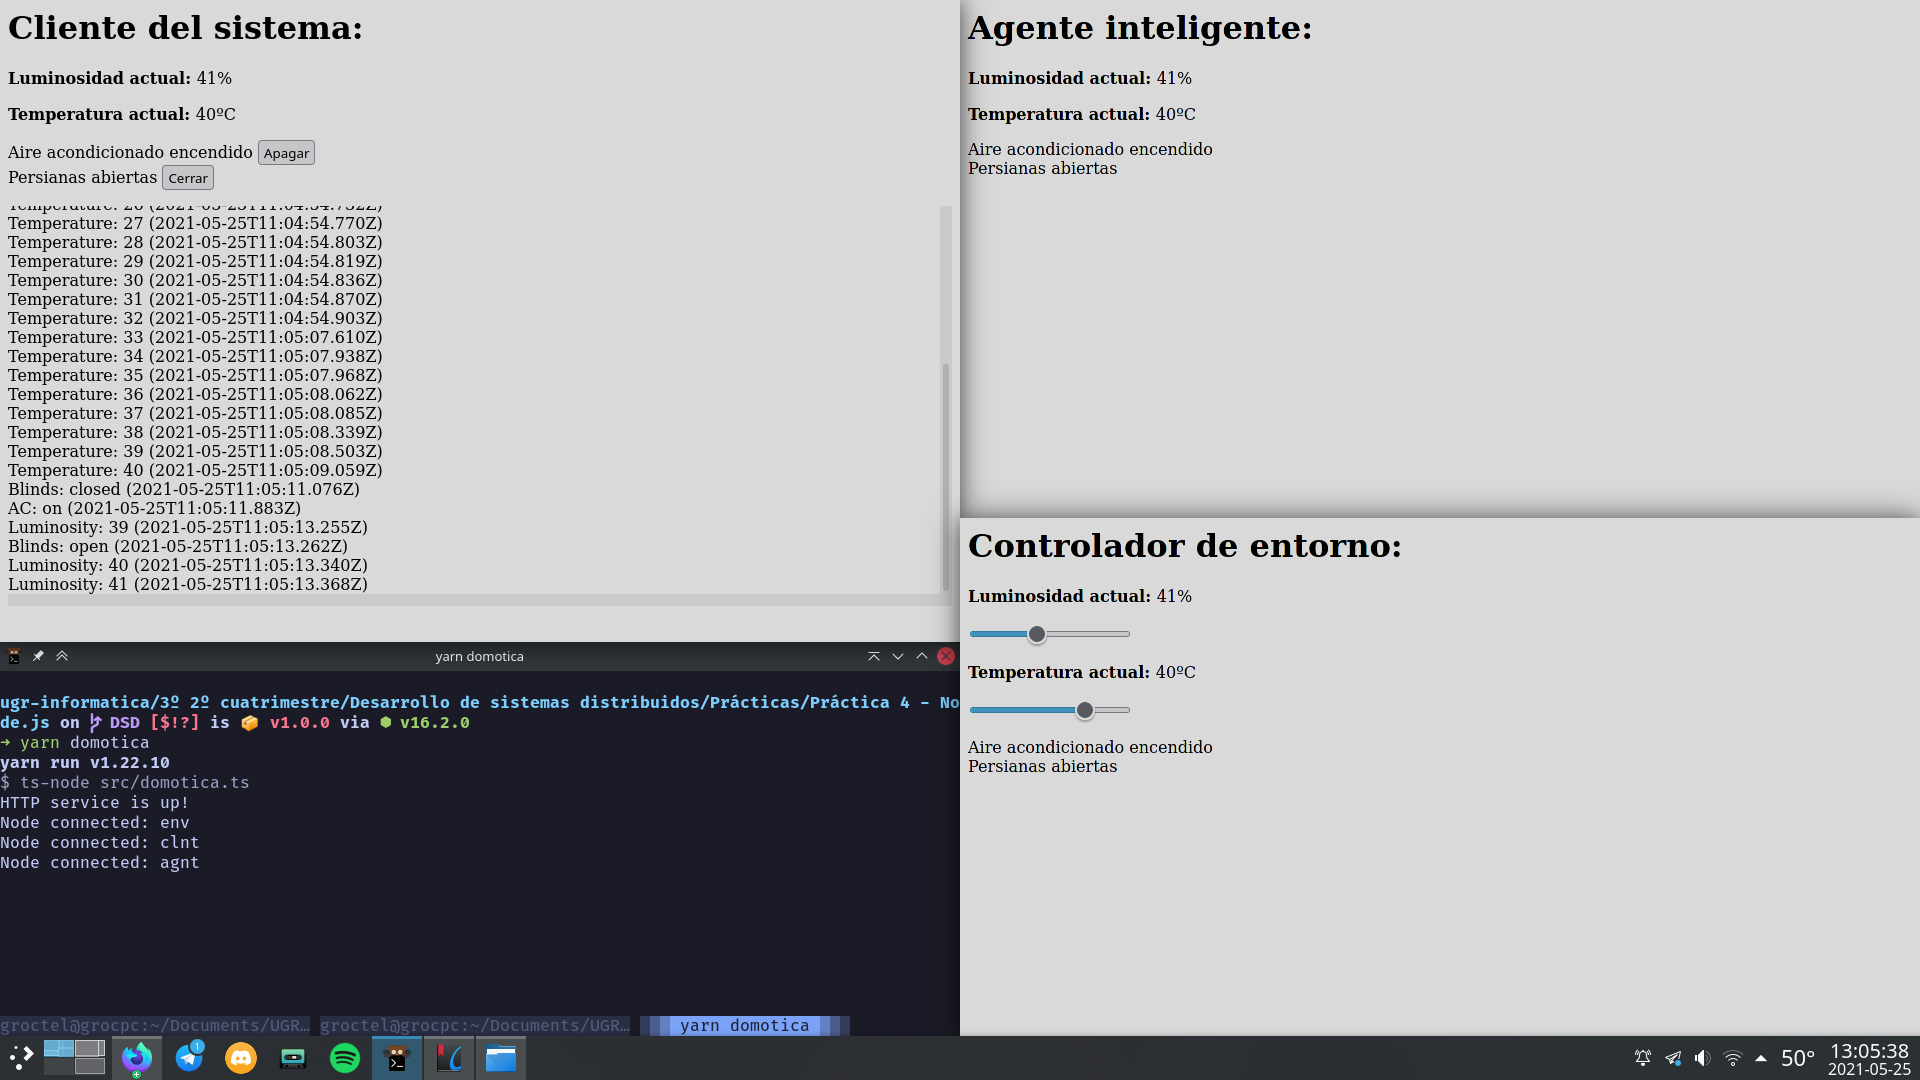
\includegraphics[scale=0.3]{node_domotica}
\end{center}
\caption{Interacción de los componentes del sistema domótico.}
\end{figure}

Este ejercicio se compone de cuatro partes:

\begin{itemize}
	\item\textbf{Servidor central:}
		Gestiona la comunicación entre los componentes del sistema.
	\item\textbf{Controlador de entorno:}
		Interfaz que simula sensores de temperatura y luminosidad.
	\item\textbf{Cliente del entorno:}
		Interfaz de usuario en la que éste puede modificar el estado de las persianas y el aire acondicionado.
	\item\textbf{Agente inteligente:}
		Cliente conectado que toma decisiones sobre el sistema y avisa al usuario de sus consecuencias.
\end{itemize}

\pagebreak

El acceso a cada uno de los nodos se hace mediante su url:

\begin{itemize}
	\item\textbf{Agente}
		\texttt{http://127.0.0.1:8080/agnt}
	\item\textbf{Cliente}
		\texttt{http://127.0.0.1:8080/clnt}
	\item\textbf{Sensores:}
		\texttt{http://127.0.0.1:8080/env}
\end{itemize}

Cuando modificamos los sensores (luminosidad y temperatura) y los sistemas (aire y persianas) los sensores y el cliente envían respectivamente una actualización de los datos al servidor central, que reenvía a todo el mundo la información con los nuevos datos.
Es decir, la interfaz desde la que se modifica el estado del sistema domótico no se actualiza hasta que el servidor central ha recibido la información y la ha transmitido con éxito.
De esta forma nos aseguramos que la información presentada en las interfaces sea la que todos los nodos han recibido.
Esto es útil porque el servidor central va guardando las actualizaciones de los sensores y los sistemas en una colección de la base de datos \texttt{mybd} del ejemplo de MongoDB, de forma que todos los clientes deben estar sincronizados a la última actualización presentada en el histórico de la base de datos.

El agente toma decisiones sencillas y avisa a los usuarios de ellas.
Si la temperatura sobrepasa los 45ºC enciende el aire y si la luminosidad llega al 80{\%} cierra las persianas.
Por otro lado, apaga el aire si la temperatura baja de 35ºC y abre las persianas si la luminosidad baja del 70{\%}.
Cuando la temperatura y la luminosidad cruzan sus máximos de 45ºC y 80{\%}, también envía una alerta a todos los clientes conectados, que se muestra en pantalla y bloquea las interfaces hasta que se resuelva usando la función \texttt{alert()}.
